%iffalse
\let\negmedspace\undefined
\let\negthickspace\undefined
\documentclass[journal,12pt,onecolumn]{IEEEtran}
\usepackage{cite}
\usepackage{amsmath,amssymb,amsfonts,amsthm}
\usepackage{algorithmic}
\usepackage{graphicx}
\usepackage{textcomp}
\usepackage{xcolor}
\usepackage{txfonts}
\usepackage{listings}
\usepackage{multicol}
\usepackage{enumitem}
\usepackage{mathtools}
\usepackage{gensymb}
\usepackage{comment}
\usepackage[breaklinks=true]{hyperref}
\usepackage{tkz-euclide} 
\usepackage{listings}
\usepackage{gvv}                                        
%\def\inputGnumericTable{}                                 
\usepackage[latin1]{inputenc}                                
\usepackage{color}                                            
\usepackage{array}                                            
\usepackage{longtable}                                       
\usepackage{calc}                                             
\usepackage{multirow}                                         
\usepackage{hhline}                                           
\usepackage{ifthen}                                           
\usepackage{lscape}
\usepackage{tabularx}
\usepackage{array}
\usepackage{float}


\newtheorem{theorem}{Theorem}[section]
\newtheorem{problem}{Problem}
\newtheorem{proposition}{Proposition}[section]
\newtheorem{lemma}{Lemma}[section]
\newtheorem{corollary}[theorem]{Corollary}
\newtheorem{example}{Example}[section]
\newtheorem{definition}[problem]{Definition}
\newcommand{\BEQA}{\begin{eqnarray}}
\newcommand{\EEQA}{\end{eqnarray}}
\newcommand{\define}{\stackrel{\triangle}{=}}
\theoremstyle{remark}
\newtheorem{rem}{Remark}

% Marks the beginning of the document
\begin{document}
\bibliographystyle{IEEEtran}
\vspace{3cm}

\title{Assignment-7}
\author{AI24BTECH11036- Shreedhanvi Yadlapally}
\maketitle

\bigskip
\renewcommand{\thefigure}{\theenumi}
\renewcommand{\thetable}{\theenumi}
\section{MCQ - 2 marks}

\begin{enumerate}

\item What should be the value of $\lambda$ such that the function defined below is continuous at $x=\frac{\pi}{2}$?\\
$f\brak{x}=
\begin{cases}
\frac{\lambda \cos x}{\frac{\pi}{2}-x} & \text{ if } x\neq \pi /2 \\
1 & \text{ if } x=\pi /2 \\
\end{cases}$
	\begin{multicols}{4}
	\begin{enumerate}
		\item 0
		\item $\frac{2}{\pi}$
		\item 1
		\item $\frac{\pi}{2}$
	\end{enumerate}
	\end{multicols}

\item What is the value of the definite integral, $\int_{0}^{a} \frac{\sqrt{x}}{\sqrt{x}+\sqrt{a-x}} dx$?
	\begin{multicols}{4}
	\begin{enumerate}
		\item 0
		\item a/2
		\item a
		\item 2a
	\end{enumerate}
	\end{multicols}

\item If $\vec{a}$ and $\vec{b}$ are two arbitrary vectors with magnitudes a nd b, respectively, $\abs{\vec{a} \times \vec{b}}^2$ will be equal to
	\begin{multicols}{4}
	\begin{enumerate}
		\item $a^{2}b^{2}-\brak{\vec{a} \cdot \vec{b}^2}^{2}$
		\item $ab-\vec{a} \cdot \vec{b}$
		\item $a^{2}b^{2}+\brak{\vec{a} \cdot \vec{b}^2}^{2}$
		\item $ab+\vec{a} \cdot \vec{b}$
	\end{enumerate}
	\end{multicols}

\item The solution of the differential equation $\frac{dy}{dx}+\frac{y}{x}=x$, with the condition that $y=1$ at $x=1$, is
	\begin{multicols}{4}
	\begin{enumerate}
		\item $y=\frac{2}{3x^{2}}+\frac{x}{3}$
		\item $y=\frac{x}{2}+\frac{1}{2x}$
 		\item $y=\frac{2}{3}+\frac{x}{3}$
		\item $y=\frac{2}{3x}+\frac{x^{2}}{3}$
	\end{enumerate}
	\end{multicols}

\item The value of $W$ that results in the collapse of the beam shown in the adjoining figure and having a plastic moment capacity of $\mathbf{M_{p}}$ is
%fig_1
\begin{figure}[ht]
\centering
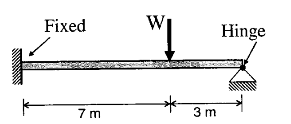
\includegraphics[scale=0.4]{figs/fig1.png}
\end{figure}
	\begin{multicols}{4}
	\begin{enumerate}
		\item (4/21)$\mathbf{M_{p}}$
		\item (3/10)$\mathbf{M_{p}}$
		\item (7/21)$\mathbf{M_{p}}$
		\item (13/21)$\mathbf{M_{p}}$
	\end{enumerate}
	\end{multicols}

\item For the cantilever bracket, PQRS, loaded as shown in the adjoining figure (PQ=RS=L, and, QR=2L), which of the following staements is \textbf{FALSE}?
%fig_2
\begin{figure}[ht]
\centering
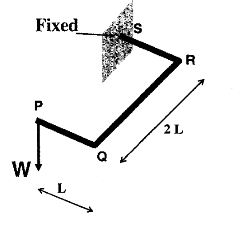
\includegraphics[scale=0.4]{figs/fig2.png}
\end{figure}
	\begin{enumerate}
		\item The portion RS has a constant twisting moment with a value of 2WL.
		\item The portion QR has a varying twisting moment with a maximum vale of WL.
		\item The portion PQ has varying bending moment with a maximum value of WL
		\item The portion PQ has no twisting moment.
	\end{enumerate}

\item Consider a bar of diameter '$D$' embedded in alarge concrete block as shown in the adjoining figure, with a pull out force $P$ being applied. Let $\sigma_b$ and $\sigma_{st}$ be the bond strength of the bar, respectively. If the block is held in position and it is assumed that the material of the block does not fail, which of the following options represents the maximum value of $P$?
%fig_3
\begin{figure}[ht]
\centering
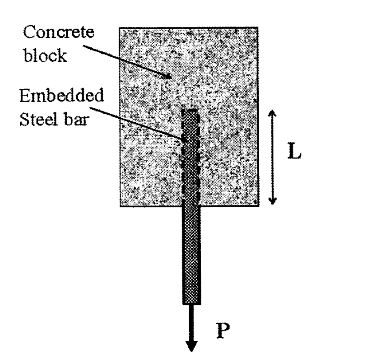
\includegraphics[scale=0.4]{figs/fig3.png}
\end{figure}
	\begin{multicols}{2}
	\begin{enumerate}
		\item Maximum of $\brak{\frac{\pi}{4}D^{2}\sigma_{b}}$ and $\brak{\pi DL\sigma_{st}}$
		\item Maximum of $\brak{\frac{\pi}{4}D^{2}\sigma_{st}}$ and $\brak{\pi DL\sigma_{b}}$
		\item Minimum of $\brak{\frac{\pi}{4}D^{2}\sigma_{st}}$ and $\brak{\pi DL\sigma_{b}}$
		\item Minimum $\brak{\frac{\pi}{4}D^{2}\sigma_{b}}$ and $\brak{\pi DL\sigma_{st}}$
	\end{enumerate}
	\end{multicols}

\item Consider two RCC beams P and Q, each having the section 400 mm $\times$ 750 mm (effective depth, d = 750 mm) made with concrete having $\tau_{\text{cmax}} = 2.1 N/mm^{2}$. For the reinforcement provided and the grade of concrete used, it may be assumed that the $\tau_c = 0.75 N/mm^{2}$. The design shear in beam P is 400 kN and in beam Q is 750 kN. Considering the provisions of IS 456-2000, which of the following statements is \textbf{TRUE}?
	\begin{enumerate}
		\item Shear reinforcement should be designed for 175 kN for beam P and the section for beam Q should be revised.
		\item Nominal shear reinforcement is required for beam P and the shear reinforcement should be designed for 120 kN for beam Q.
		\item Shear reinforcement should be designed for 175 kN for beam P and the shear reinforcement should be designed for 525 kN for beam Q.
		\item The sections for both beams P and Q need to be revised.
	\end{enumerate}

\item The adjoining figure shows a schematic representation of a steel plate girder to be used as asimply supported beam with a concentrated load. For stiffeners, PQ (running along the beam axis) and RS (running between the top and bottom flanges) which of the following pairs of statements will be \textbf{TRUE}?
%fig_4
\begin{figure}[ht]
\centering
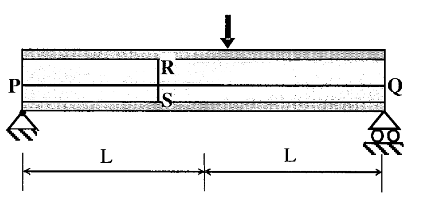
\includegraphics[scale=0.4]{figs/fig4.png}
\end{figure}
	\begin{enumerate}
		\item \begin{enumerate}
				\item RS should be provided under the concentrated load only.
				\item PQ should be placed in the tension side of the flange
			\end{enumerate}
		\item \begin{enumerate}
				\item RS helps to prevent local buckling of the web.
				\item PQshould be placed on the compression side of the flange.
			\end{enumerate}
		\item \begin{enumerate}
				\item RS should be provided at supports.
				\item PQ should be placed along the neutral axis.
			\end{enumerate}
		\item \begin{enumerate}
				\item RS should be provided away from points of action of concentrated loads.
				\item PQ should be provided on the compression side of the flange.
			\end{enumerate}
	\end{enumerate}

\item A singly under-reamed, 8-m long RCC pile (shown in the adjoining figure) weighing 20 kN with 350 mm shaft diameter and 750 mm under-ream diameter is installed within stiff, saturated silty clay (undrained shear strength is 50 kPa, adhesion factor is 0.3, and the applicable bearing capacity factor is 9) to counteract the impact of soil swelling on a structure constructed above. Neglecting suction and the contribution of the under-ream to the adhesive shaft capacity, what would be the estimated ultimate tensile capacity (rounded off to the nearest integer value of kN) of the pile?
	%fig_5
\begin{figure}[ht]
\centering
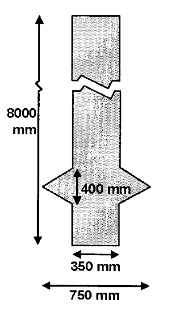
\includegraphics[scale=0.4]{figs/fig5.png}
\end{figure}
	\begin{multicols}{4}
	\begin{enumerate}
		\item 132 kN
		\item 156 kN
		\item 287 kN
		\item 301 kN
	\end{enumerate}
	\end{multicols}

\item Identical surcharges are placed at ground surface at site $X$ and $Y$, wuth soil conditions shown alongside and water table at ground surface. The silty clay layers at $X$ and $Y$ are identical. THe thin sand layer at $Y$ is continuous and free-drai ning with a very large discharge capacity. If primary consolidation at $X$ is estimated to complete in 36 months, what would be the corresponding time for completion of primary consolidation at $Y$?
%fig_6
\begin{figure}[ht]
\centering
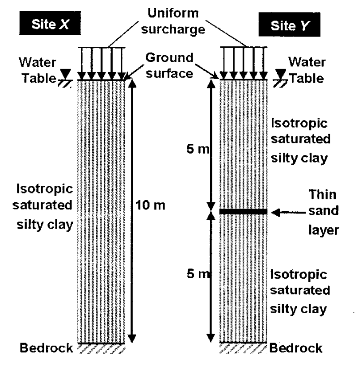
\includegraphics[scale=0.4]{figs/fig6.png}
\end{figure}
	\begin{multicols}{4}
	\begin{enumerate}
		\item 2.25 months
		\item 4.5 months
		\item 9 months
		\item 36 months
	\end{enumerate}
	\end{multicols}

\item A field vane shear testing instrument (shown alongside) was inserted completely into a deposit of soft, saturated silty clay with the vane rod vertical such that the top of the blades were 500 mm below the ground surface. Upon application of a rapidly increasing torque about the vane rod, the soil was found to fail when the torque reached 4.6 Nm. Assuming mobilization of undrained shear strength on all failure surfaces to be negligible, what would be the peak undrained shear strength (rounded off to the nearest integere value of kPa) of the soil?
%fig_7
\begin{figure}[ht]
\centering
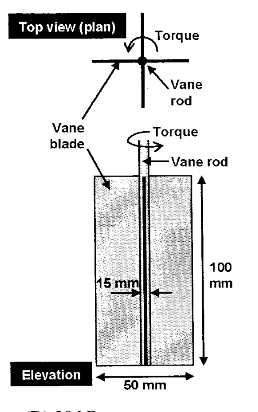
\includegraphics[scale=0.4]{figs/fig7.png}
\end{figure}
	\begin{multicols}{4}
	\begin{enumerate}
		\item 5 kPa
		\item 10 kPa
		\item 15 kPa
		\item 20 kPa
	\end{enumerate}
	\end{multicols}

\item A single pipe of length 1500 m and diameter 60 cm connects two resevoirs having a difference of 20 m in their water levels. The pipe is to be replaced by two pipes of the same length and equal diameter $d$ to convey 25\% more discharge under the same head loss. If the friction factor is assumed to be the same for all the pipes, the value of $d$ is approximately equal to which of the following options?
	\begin{multicols}{4}
	\begin{enumerate}
		\item 37.5 cm
		\item 40.0 cm
		\item 45.0 cm
		\item 50.0 cm
	\end{enumerate}
	\end{multicols}

\end{enumerate}
\end{document}
